\section{Further W+MET models with possible cross-section enhancements} 

%Contributed by Yang Bai

As pointed out in Ref.~\cite{Bell:2015sza}, the mono-$W$ signature can probe the iso-spin violating interactions of dark matter with quarks. The relevant operators after the electroweak symmetry breaking is 
%
\begin{equation}
\frac{1}{\Lambda^2}\overline{\chiDM} \gamma_\mu \chiDM \left( \overline{u}_L \gamma^\mu u_L + \xi \bar{d}_L \gamma^\mu d_L \right) \,.
\end{equation}
%
Here, we only keep the left-handed quarks because the right-handed quarks do not radiate a $W$-gauge boson from the weak interaction. As the LHC constraints the cutoff to higher values, it is also important to know the corresponding operators before the electroweak symmetry. At the dimension-six level, the following operator
%
\begin{equation}
\frac{c_6}{\Lambda^2}\overline{\chiDM} \gamma_\mu \chiDM \,\overline{Q}_L \gamma^\mu Q_L 
\end{equation}
%
conserves iso-spin and provides us $\xi=1$~\cite{Bell:2015sza}. At the dimension-eight level, new operators appear to induce iso-spin violation and can be
%
\begin{equation}
\frac{c^d_8}{\Lambda^4}\overline{\chiDM} \gamma_\mu \chiDM \,(H\overline{Q}_L) \gamma^\mu (Q_L H^\dagger) 
+ \frac{c^u_8}{\Lambda^4}\overline{\chiDM} \gamma_\mu \chiDM \,(\tilde{H}\overline{Q}_L) \gamma^\mu (Q_L \tilde{H}^\dagger)  \,.
\end{equation}
% 
After inputting the vacuum expectation value of the Higgs field, we have 
\begin{equation}
\xi = \frac{c_6 \,+\, c_8^d\,v_{\rm EW}^2/2\Lambda^2}{c_6 \,+\, c_8^u \,v_{\rm EW}^2/2\Lambda^2} \,.
\end{equation}
% 
For a nonzero $c_6$ and $v_{\rm EW} \ll \Lambda$, the iso-spin violation effects are suppressed. On the other hand, the values of $c_6$, $c^d_8$ and $c^u_8$ depend on the UV-models. 

There is one possible UV-model to obtain a zero value for $c_6$ and non-zero values for $c^d_8$ and $c^u_8$. One can have the dark matter and the SM Higgs field charged under a new $U(1)^\prime$. There is a small mass mixing between SM $Z$-boson and the new \Zprime with a mixing angle of ${\cal O}(v_{\rm EW}^2/M^2_{\Zprime})$. After integrating out \Zprime, one has different effective dark matter couplings to $u_L$ and $d_L$ fields, which are proportional to their couplings to the $Z$ boson. For this model, we have $c_6=0$ and 
 %
\begin{equation}
\xi = \frac{-\frac{1}{2} + \frac{1}{3} \sin^2{\theta_W} }{ \frac{1}{2} - \frac{2}{3} \sin^2{\theta_W}} \approx  -2.7 
\end{equation}
%
and order of unity. 

\section{Simplified model corresponding to dimension-5 EFT operator}

% +++++++++++++++++++++++++++++++++++++++++++++++++++++++++++++++++++++++++++++++++++++
%   Linda 11/5/15
% +++++++++++++++++++++++++++++++++++++++++++++++++++++++++++++++++++++++++++++++++++++

As an example of a simplified model corresponding to the dimension-5 EFT operator 
described in Section~\ref{sec:EFT_models_with_direct_DM_boson_couplings}, 
we consider a Higgs portal with a scalar mediator. Models of this kind
are among the most concise versions of simplified models that produce 
couplings of Dark Matter to pairs of gauge-bosons.  Scalar fields may couple directly to pairs of electroweak gauge bosons, 
but must carry part of the electroweak vacuum expectation value.  One may thus consider a simple model where Dark Matter couples to a a scalar 
singlet mediator, which mixes with the fields in the Higgs sector.
\begin{equation}
L\subset m_s S^2 + \lambda S^2H^2 +\lambda^{'} S H^2 + y S \chiDM \overline{\chiDM}
\end{equation}
Where H is a field in the Higgs sector that contains part of the electroweak vacuum expectation value, 
S is a heavy scalar singlet and $\chiDM$ is a Dark Matter field. 
There is then an S channel diagram where DM pairs couple to the singlet field S, 
which then mixes with a Higgs-sector field, and couples to W and Z bosons. 
This diagram contains 2 insertions of EW symmetry breaking fields, 
corresponding in form to the effective dimension-5 operator in Section~\ref{sub:EW_EFT_Dim5}.   

\section{Inert 2HDM Model}\label{sec:i2HDM}

For most of the simplified models included in this report, the mass of
the mediator and couplings/width are non-trivial parameters of the
model. In these scenarios, we remain agnostic about the theory behind
the dark matter sector and try to parametrize it in simple terms.

We have not addressed how to extend the simplified models to realistic
and viable models which are consistent with the symmetries of the
Standard Model. Simplified models often violate gauge invariance which
is a crucial principle for building a consistent BSM model which
incorporates SM together with new physics. For example, with a new
heavy gauge vector boson mediating DM interactions, one needs not just
the dark matter and its mediator, but also a mechanism which provides
mass to this mediator in a gauge invariant way.

Considering both the simplified model and other elements necessary for a consistent theory is a next logical step. The authors of \cite{Belyaev:2015tap} term these Minimal
Consistent Dark Matter (MCDM) models. MCDM models are at the same time still toy models that can be 
easily incorporated into a bigger BSM model and explored via
complementary constraints from collider and direct/indirect DM search
experiments as well as relic density constraints. We discuss this model here both on its own merits and as an example of the flexibility of the simplified model approach.

The idea of an inert Two-Higgs Doublet Model (i2HDM) was introduced
more than 30 years ago in~\cite{Deshpande:1977rw,LopezHonorez:2006gr,Dolle:2009fn,Goudelis:2013uca,Balyaev:2015tap}. It is an extension of the SM with a second scalar doublet $\phi_2$ with no direct coupling to fermions.  This doublet has a discrete $Z_2$ symmetry, under which $\phi_2$ is odd and all the other fields are even. 
The Lagrangian of the odd sector is,
  \begin{equation}
  \mathcal{L} = \frac{1}{2}(D_{\mu}\phi_2)^2 -V(\phi_1,\phi_2)
  \end{equation}
with the  potential $V$  containing mass terms and $\phi_1 - \phi_2$
interactions:
\begin{eqnarray}
  V &=& -m_1^2 (\phi_1^{\dagger}\phi_1) - m_2^2 (\phi_2^{\dagger}\phi_2) + \lambda_1 (\phi_1^{\dagger}\phi_1)^2 + \lambda_2 (\phi_2^{\dagger}\phi_2)^2    \nonumber  \\
  &+&  \lambda_3(\phi_2^{\dagger}\phi_2)(\phi_1^{\dagger}\phi_1)  + \lambda_4(\phi_2^{\dagger}\phi_1)(\phi_1^{\dagger}\phi_2) + 
  \frac{\lambda_5}{2}\left[(\phi_1^{\dagger}\phi_2)^2 + (\phi_2^{\dagger}\phi_1)^2 \right],
\end{eqnarray}
where $\phi_1$ and  $\phi_2$ are SM and inert Higgs doublets respectively carrying the same hypercharge. These doublets can be parameterised as
\begin{equation}
\phi_1=\frac{1}{\sqrt{2}}
\begin{pmatrix}
0\\
v+H 
\end{pmatrix}
  \qquad
  \phi_2= \frac{1}{\sqrt{2}}
\begin{pmatrix}
 \sqrt{2}{h^+} \\
 h_1 + ih_2
\end{pmatrix}
\end{equation}

In addition to the SM, i2HDM brings four more degrees of
freedom coming from the inert doublet in the form of $Z_2$-odd charged
scalar $\textrm{h}^\pm$ and two neutral $Z_2$-odd scalars
$\textrm{h}_1$ and $\textrm{h}_2$. The lightest neutral scalar, $h_1$
is identified as the dark matter candidate. The i2HDM model has been explored at the
phenomenological level from the perspective of collider DM searches
\cite{Burgess:2000yq, Andreas:2008xy, Arhrib:2013ela, Belyaev:2015tap}. This model could produce \MET+jet, Z, and Higgs as well as \MET+VBF signatures at the LHC (see Figs.~\ref{fig:fd-monojet1,fig:fd-monojet2,fig:fd-mono-Z,fd:mono-H1,fd:mono-H2,fd-vbf}).

\begin{figure}
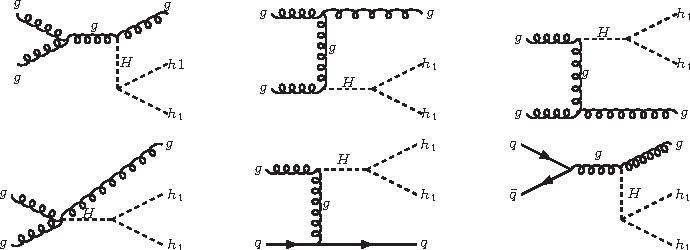
\includegraphics[width=\textwidth]{figures/EW/i2HDM/fd-mono-j1.pdf} 
\caption{Feynman diagrams for $gg\to h_1 h_1+g$ process
contributing to mono-jet signature.}
\label{fig:fd-monojet1}
\end{figure}
\begin{figure}[htb]
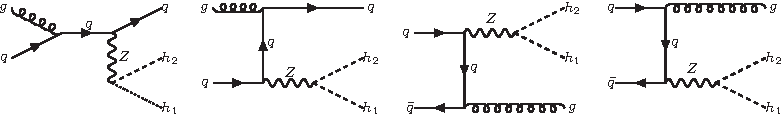
\includegraphics[width=\textwidth]{figures/EW/i2HDM/fd-mono-j2.pdf} 
\caption{Feynman diagrams for $q\bar{q}\to h_1 h_2+g$ ($gq\to h_1 h_2+q$) process 
contributing to mono-jet signature.}
\label{fig:fd-monojet2}
\end{figure}
\begin{figure}[htb]
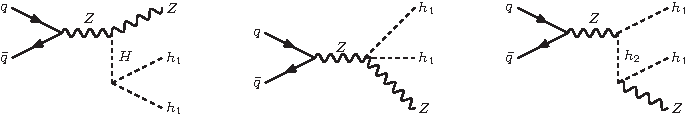
\includegraphics[width=\textwidth]{figures/EW/i2HDM/fd-mono-z.pdf} 
\caption{Feynman diagrams for $q\bar{q}\to h_1 h_1+Z$  process 
contributing to mono-Z signature.}
\label{fig:fd-mono-Z}
\end{figure}
\begin{figure}[htb]
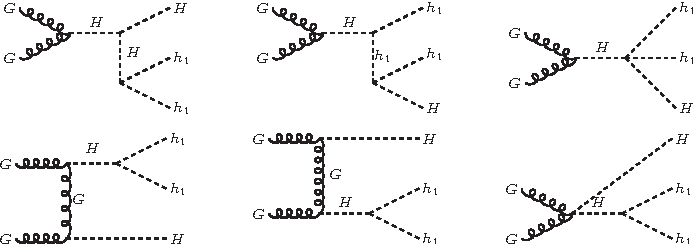
\includegraphics[width=\textwidth]{figures/EW/i2HDM/fd-mono-h1.pdf} 
\caption{Feynman diagrams for $gg\to h_1 h_1+H$  process 
contributing to mono-Higgs signature.}
\label{fig:fd-mono-H1}
\end{figure}
\begin{figure}[htb]
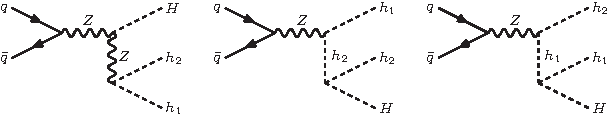
\includegraphics[width=\textwidth]{figures/EW/i2HDM/fd-mono-h2.pdf} 
\caption{Feynman diagrams for $q\bar{q}\to h_1 h_2+H$  process 
contributing to mono-Higgs signature.}
\label{fig:fd-mono-H2}
\end{figure}
\begin{figure}[htb]
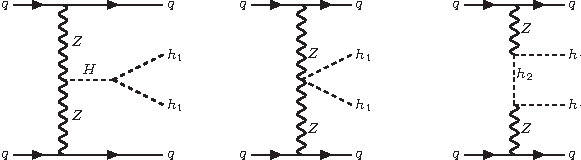
\includegraphics[width=\textwidth]{figures/EW/i2HDM/fd-vbf.pdf} 
\caption{Diagrams for $qq\to qq h_1 h_1$ DM production in vector boson
fusion process}
\label{fig:fd-vbf}
\end{figure}

An experimental analysis of the parameter space has recently been
performed in Ref.~\cite{Belyaev:2015tap}. The authors of that study
have implemented the model in CalcHEP and micrOMEGAs and propose a set
of benchmark points (Table.~\ref{tab:i2HDMbenchMarks}). Though the
overall parameter space of i2HDM is 5-dimensional, the parameter space
relevant to a specific LHC signature is only 1-2 dimensional. In the
mono-jet case, one can use two separate simplified models, a
$gg\to h_1 h_1+g$ process (via Higgs mediator) and a
$q\bar{q}\to h_1 h_2+g$ ($gq\to h_1 h_2+q$) process (using Z-boson
mediator) to capture the physics relevant to the search.

\begin{table*}[htb]
\centering
\begin{tabular}{|c||c|c|c|c|c|c|}
\hline
 {\bf BM}                       &  {\bf 1}  & {\bf 2}  & {\bf 3}  & {\bf 4}  &  {\bf 5}  \\
  \hline\hline 
  $M_{h_{1}}$ (GeV)     & 45 & 53 & 66 & 82 & 120 \\ 
  \hline
  $M_{h_{2}}$ (GeV)     &  55  & 189  &  77  &  89  & 140 \\
  \hline
  $M_{h_{\pm}}$ (GeV)  & 130 & 182  &  122  &  150  &  200 \\
  \hline
  $\lambda_{2}$             &  0.8 & 1.0 & 1.1 & 0.9 & 1.0 \\  
  \hline
  $\lambda_{345}$         & $-0.010$ & $-0.024$  & $+0.022$ & $-0.090$  & $-0.100$      \\
  \hline
  $\Omega^{2}_{h}$       & $1.1 \times 10^{-1}$ &  $8.1 \times 10^{-2}$  & $9.9 \times 10^{-2}$  & $1.5 \times 10^{-2}$  &  $2.1 \times 10^{-3}$ \\
  \hline 
  $\sigma_{SI}$ (fb)        & $1.9 \times 10^{-7}$ &  $7.9 \times 10^{-7}$  & $4.2 \times 10^{-7}$  & $4.5 \times 10^{-7}$  &  $2.6 \times 10^{-6}$ \\
 \hline 
  $\sigma_{LHC}$ (fb)     & $1.7 \times 10^{2}$ &  $7.7 \times 10^{2}$  & $4.3 \times 10^{-2}$  & $1.2 \times 10^{-1}$  &  $2.3 \times 10^{-2}$ \\
  \hline\hline
\end{tabular}
\caption{Five benchmarks (BM) for i2HDM in  ($M_{h_{1}},M_{h_{2}},M_{h_{\pm}},\lambda_{2},\lambda_{345}$) parameter space.
 We also present the corresponding relic density ($\Omega_{h^2}$), the spin-independent cross section for DM scattering on the proton,
 and the LHC cross section at 13 TeV for mono-jet process $pp\to h_1,h_1+jet$ for $p_T^{jet}>100$~GeV cut.}
\label{tab:i2HDMbenchMarks}
\end{table*}
\clearpage

\section{Tabulated cross-sections}

\subsection{photon+MET signal, \schannel vector mediator model}

\subsection{Higgs+MET signal, vector mediator model}

Figure~\ref{fig:zprimeXS} shows the cross sections in this vector mediator model in the $m_{med}$ 
vs $m_{DM}$ plane. The tabulated values can be found in Table~\ref{tab:zprimeXS}

\begin{figure}[hbpt!]
	\begin{center}
		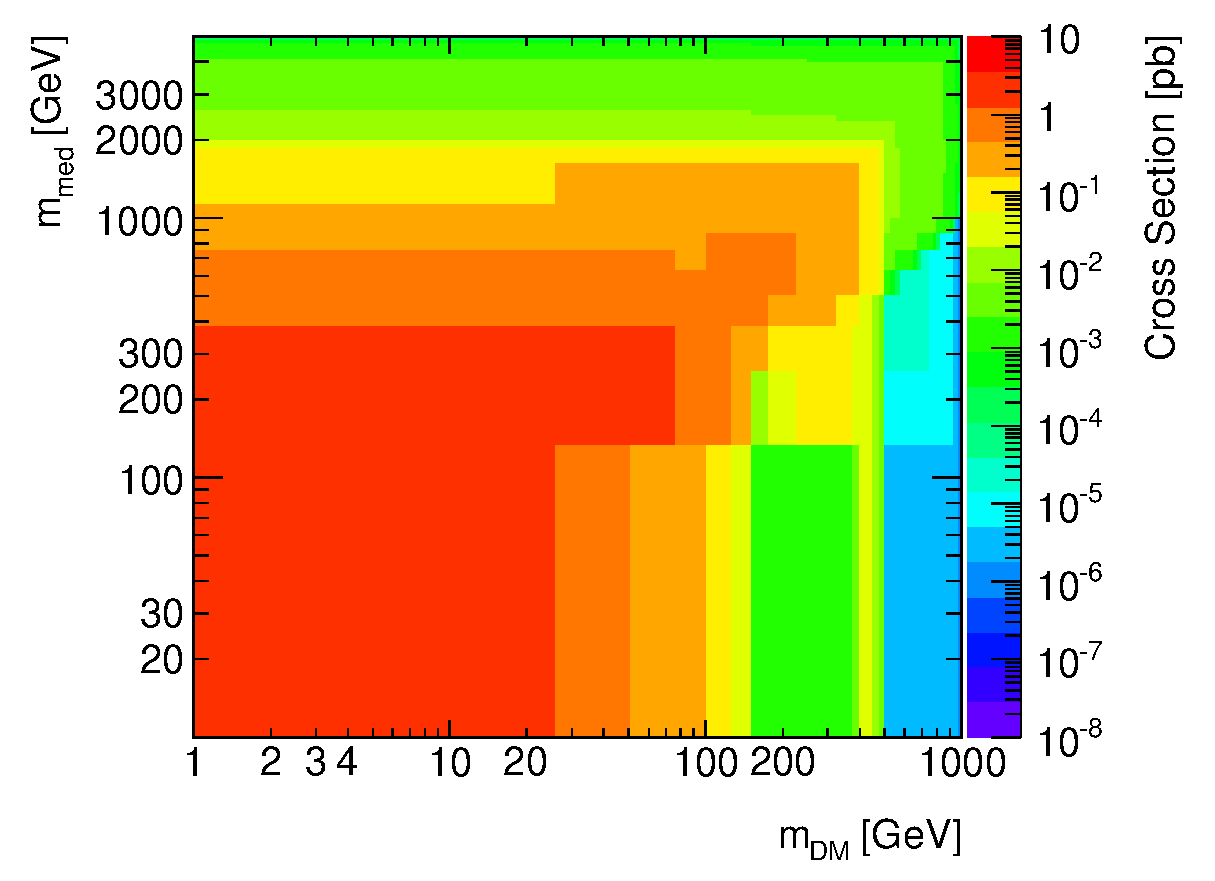
\includegraphics[width=0.9\linewidth]{figures/EW/monoH/zprime_cross_section_new}
		\caption{ Cross section of the $pp \rightarrow H\chiDM\bar{\chiDM}$ process 
			in units of pico-barn for the vector mediator model. 
			\label{fig:zprimeXS}}
	\end{center}
\end{figure}


\begin{table}
	\centering
	\begin{tabular}{ccc}
		$m_{DM}$ [GeV] & $m_{med}$ [GeV] & $\sigma_{pp\rightarrow h\chiDM\bar{\chiDM}}$ [pb] \\ \hline
		1 & 10 & 0.0003835 \\
		1 & 20 & 0.0003177 \\
		1 & 50 & 0.0001467 \\
		1 & 100 & 0.0001065 \\
		1 & 200 & 6.867e-05 \\
		1 & 300 & 7.388e-05 \\
		1 & 500 & 7.858e-05 \\
		1 & 1000 & 4.327e-05 \\
		1 & 2000 & 4.018e-05 \\
		1 & 5000 & 3.336e-05 \\ \hline
		10 & 10 & 3.603e-06 \\
		10 & 15 & 1.477e-05 \\
		10 & 50 & 0.0001547 \\
		10 & 100 & 0.0001104 \\
		10 & 5000 & 4.5e-05 \\ \hline
		50 & 10 & 1.401e-07 \\
		50 & 50 & 2.099e-07 \\
		50 & 95 & 2.813e-05 \\
		50 & 200 & 4.82e-05 \\
		50 & 300 & 7.485e-05 \\
		50 & 5000 & 3.384e-05 \\ \hline
		150 & 10 & 4.833e-09 \\
		150 & 295 & 3.65e-08 \\
		150 & 500 & 6.463e-07 \\
		150 & 5000 & 2.407e-08 \\ \hline
		500 & 10 & 8.672e-12 \\
		500 & 500 & 1.157e-11 \\
		500 & 995 & 5.254e-10 \\
		500 & 2000 & 7.138e-10 \\
		500 & 5000 & 5.87e-10 \\ \hline
		1000 & 10 & 5.946e-14 \\
		1000 & 1000 & 1.546e-13 \\
		1000 & 1995 & 8.316e-12 \\
		1000 & 5000 & 2.112e-11 \\ \hline
	\end{tabular}
	\caption{ Cross section of the $pp \rightarrow h\chiDM\bar{\chiDM}$ process 
		in units of pico-barn for the vector mediator model. 
		\label{tab:zprimeXS}}
\end{table}

\subsection{Higgs+MET signal, scalar mediator model}

Figure~\ref{fig:scalarXS} shows the cross sections of the $pp \rightarrow H\chiDM\bar{\chiDM}$ process 
in this vector mediator model in the $m_{med}$ 
vs $m_{DM}$ plane. The tabulated values can be found in Table~\ref{tab:scalarXS}

\begin{figure}[hbpt!]
	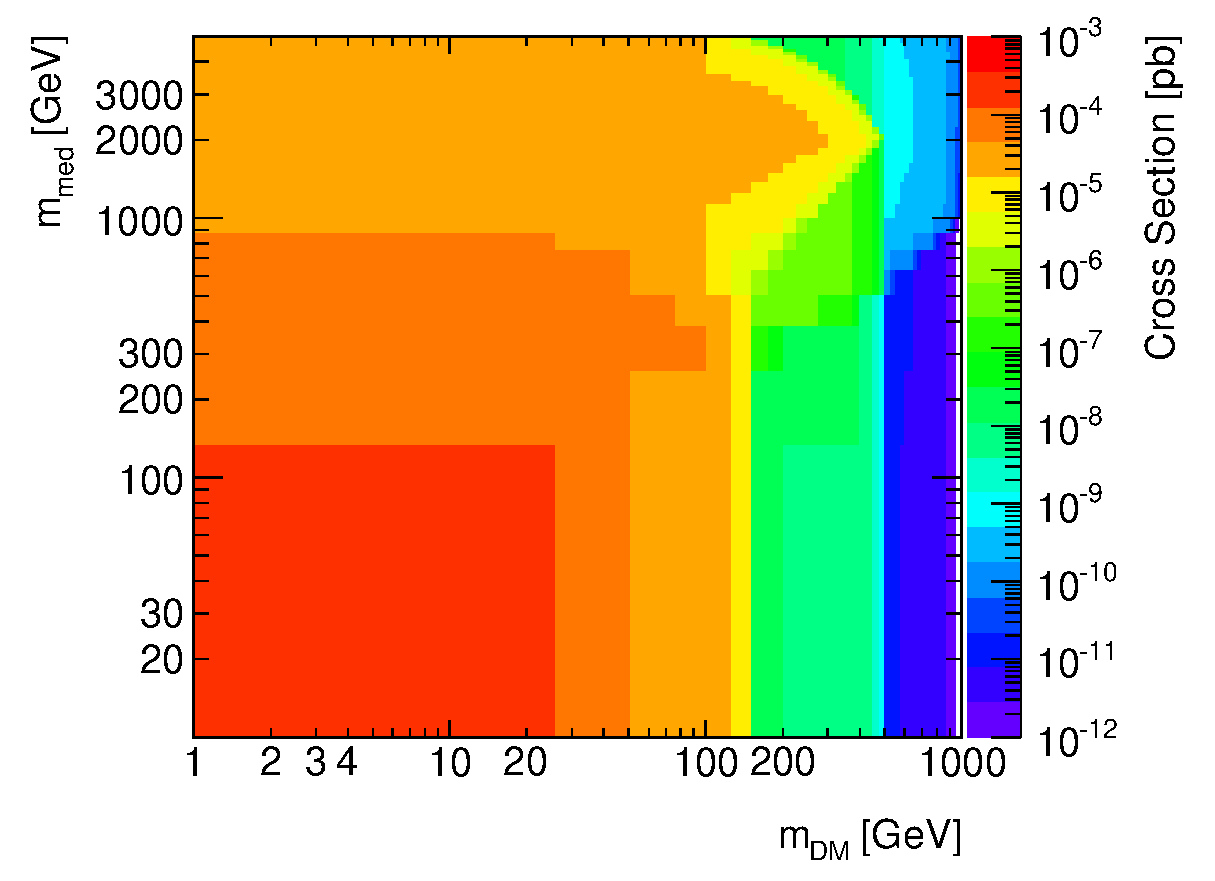
\includegraphics[width=0.8\linewidth]{figures/EW/monoH/scalar_cross_section_new}
	\caption{ \label{fig:scalarXS} Cross section of the $pp \rightarrow H\chiDM\bar{\chiDM}$ process 
		in units of pico-barn for the scalar mediator model.}
\end{figure}

\begin{table}
	\centering
	\begin{tabular}{ccc}
		$m_{DM}$ [GeV] & $m_{med}$ [GeV] & $\sigma_{pp\rightarrow h\chiDM\bar{\chiDM}}$ [pb] \\ \hline
		1 & 10 & 2.389 \\
		1 & 20 & 2.483 \\
		1 & 50 & 2.98 \\
		1 & 100 & 2.881 \\
		1 & 200 & 2.344 \\
		1 & 300 & 2.041 \\
		1 & 500 & 0.9328 \\
		1 & 1000 & 0.1524 \\
		1 & 2000 & 0.008919 \\
		1 & 5000 & 1.39e-05 \\ \hline
		10 & 10 & 0.01895 \\
		10 & 15 & 0.7378 \\
		10 & 50 & 2.929 \\
		10 & 100 & 2.875 \\
		10 & 5000 & 1.387e-05 \\ \hline
		50 & 10 & 0.0003215 \\
		50 & 50 & 0.01127 \\
		50 & 95 & 0.2784 \\
		50 & 200 & 1.868 \\
		50 & 300 & 1.759 \\
		50 & 5000 & 1.391e-05 \\ \hline
		150 & 10 & 4.786e-06 \\
		150 & 200 & 0.004841 \\
		150 & 295 & 0.156 \\
		150 & 500 & 0.575 \\
		150 & 5000 & 1.391e-05 \\ \hline
		500 & 10 & 6.296e-09 \\
		500 & 500 & 2.855e-05 \\
		500 & 995 & 0.008244 \\
		500 & 2000 & 0.007899 \\
		500 & 5000 & 1.355e-05 \\ \hline
		1000 & 10 & 3.78e-11 \\
		1000 & 1000 & 7.372e-07 \\
		1000 & 1995 & 0.0004346 \\
		1000 & 5000 & 1.245e-05 \\ \hline
	\end{tabular}
	\caption{ \label{tab:scalarXS} Cross section of the $pp \rightarrow h\chiDM\bar{\chiDM}$ process 
		in units of pico-barn for the scalar mediator.}
\end{table}


\subsection{Higgs+MET signal from 2HDM model with a \Zprime and a new pseudoscalar}
\label{subsec:Simulation}

The leading order cross-sections from the \madgraph generator for the signal samples are listed in Tables~\ref{tab:SigSamplesZpA0}, ~ \ref{tab:SigSamplesZpDM}, ~ \ref{tab:SigSamplesZpZh}, for the various scan points recommended.  

\begin{table}
	\centering
	\small
	\begin{tabular}{|c|c|c|}
		\hline
		$M_{\Zprime}$ (GeV) & $M_{A^0}(GeV)$ & $\sigma$ [pb] \\ \hline \hline
		600 & 300 & 1.55E-01  \\
		600 & 400 & 2.18E-02  \\
		800 & 300 & 8.30E-02  \\
		800 & 400 & 2.72E-02  \\
		800 & 500 & 1.09E-02  \\
		800 & 600 & 2.98E-03  \\
		1000 & 300 & 3.74E-02  \\
		1000 & 400 & 1.53E-02  \\
		1000 & 500 & 8.91E-03  \\
		1000 & 600 & 4.89E-03  \\
		1000 & 700 & 2.21E-03  \\
		1000 & 800 & 7.05E-04  \\
		1200 & 300 & 1.70E-02  \\
		1200 & 400 & 7.65E-03  \\
		1200 & 500 & 5.14E-03  \\
		1200 & 600 & 3.52E-03  \\
		1200 & 700 & 2.25E-03  \\
		1200 & 800 & 1.27E-03  \\
		1400 & 300 & 8.00E-03  \\
		1400 & 400 & 3.79E-03  \\
		1400 & 500 & 2.75E-03  \\
		1400 & 600 & 2.09E-03  \\
		1400 & 700 & 1.58E-03  \\
		1400 & 800 & 1.06E-03  \\
		\hline
		\hline
	\end{tabular}
	\caption{LO cross-sections for $\Zprime \to A^0h$ samples, varying $M_{\Zprime}$ and $M_{A^0}$, keeping the DM mass fixed to 100 GeV. 
    The columns from left to right describe $M_{\Zprime}$, $M_{A^0}$ and the sample cross section in pb.}
   \label{tab:SigSamplesZpA0}
\end{table}

\begin{table}
	\centering
	\small
	\begin{tabular}{|c|c|c|c|}
		\hline
		$M_{\Zprime}$ (GeV) & $M_{A^0}(GeV)$ & $M_{DM} (GeV)$ & $\sigma$ [pb] \\ \hline \hline
		1000 & 300 & 10 & 3.76E-02  \\
		1000 & 300 & 50 & 3.75E-02  \\
		1200 & 600 & 10 & 3.64E-03  \\
		1200 & 600 & 20 & 3.07E-03  \\
		\hline
		\hline
	\end{tabular}
	\caption{LO cross-sections for $\Zprime \to A^0h$ samples, when varying $M_{DM}$. The columns from left to right describe $M_{\Zprime}$, $M_{A^0}$, $M_{DM}$, and the sample cross section in pb.}
	\label{tab:SigSamplesZpDM}
\end{table}

\begin{table}
	\centering
	\small
	\begin{tabular}{|c|c|}
		\hline
		$M_{\Zprime}$ (GeV) & $\sigma$ [pb] \\ \hline \hline
		600 & 1.15E-01  \\
		800 & 3.21E-02  \\
		1000 & 1.13E-02  \\
		1200 & 4.54E-03  \\
		1400 & 2.00E-03  \\
		\hline
		\hline
	\end{tabular}
	\caption{LO cross-sections for $\Zprime \to Zh$ exclusive samples, varying $M_{\Zprime}$. The columns from left to right describe $M_{\Zprime}$ and the sample cross section in pb.}
	\label{tab:SigSamplesZpZh}
\end{table}
